\documentclass[reprint,english,notitlepage]{revtex4-1}

\usepackage[utf8]{inputenc}
\usepackage[english]{babel}
\usepackage{physics,amssymb}
\usepackage{graphicx}
\usepackage{xcolor}
\usepackage{hyperref}
\usepackage{tikz}
\usepackage{listings}
\usepackage{subfigure}

% defines the color of hyperref objects
% Blending two colors:  blue!80!black  =  80% blue and 20% black
\hypersetup{
	colorlinks,
	linkcolor={red!50!black},
	citecolor={blue!50!black},
	urlcolor={blue!80!black}
}

%% Defines the style of the programming listing
\lstset{
	inputpath=,
	backgroundcolor=\color{white!95!black},
	basicstyle={\ttfamily\scriptsize},
	commentstyle=\color{magenta},
	language=Python,
	morekeywords={True,False},
	tabsize=4,
	stringstyle=\color{green!55!black},
	frame=single,
	keywordstyle=\color{blue},
	showstringspaces=false,
	columns=fullflexible,
	keepspaces=true
}

\begin{document}
\title{Seksjon 1A: Modelering av en rakettmotor og simulering av en rakettoppskytning}
\author{Bendik og Ole Kristian}
\date{\today}
\noaffiliation                % ignore this
\begin{abstract}
	Hmmm, føer at denne rapporten er ganske abstrakt egentlig
\end{abstract}
\maketitle                    % creates the title, author, date & abstract

% the fundamental components of scientific reports:
\section{Introduction}
	Denne rapporten handler om modelering av en rakettmotor, og hvordan resultatet
	kan brukes til å modelere en rakettoppskytning. Grunnen til at vi skal gjøre dette
	er fordi vi vil etterhvert komme oss til en annen planet. Vi skyter opp raketten
	fra en planet i et tilfeldig generert solsystem til, og skal komme oss til
	en annen planet i dette solsystemet. Her er noen relevante verdier til det
	tilfeldig genererte solsystemet:

	\begin{table}[h]
		\caption{Solsystemverdier}\label{solartable}
		\makebox[0.4\textwidth][c]{
			\begin{tabular}{|c|c|c|c|c|}
				\hline
				Navn & Type & Masse & Radius & Rotasjonshastighet\\
				\hline
				Solen & Sol & 5.61$\cdot10^{29}$ kg & 280740 km & ukjent \\
				\hline
				Hjemplanet & Stein & 1.82$\cdot10^{25}$ kg & 9572 km & 6.37$\cdot10^{-5}$ 1/s \\
				\hline
				Planet 2 & Stein & 6.94$\cdot10^{24}$ kg & 6457 km & 8.51$\cdot10^{-5}$ 1/s \\
				\hline
				Planet 3 & Gass & 3.31$\cdot10^{27}$ kg & 76942 km & 1.25$\cdot10^{-4}$ 1/s \\
				\hline
				Planet 4 & Stein & 1.4$\cdot10^{22}$ kg & 826 km & 2.1$\cdot10^{-6}$ 1/s \\
				\hline
				Planet 5 & Stein & 1.6$\cdot10^{24}$ kg & 3906 km & 2.49$\cdot10^{-6}$ 1/s \\
				\hline
				Planet 6 & Gass & 3.28$\cdot10^{25}$ kg & 20050 km & 2.54$\cdot10^{-4}$ 1/s \\
				\hline
				Planet 7 & Stein & 7.64$\cdot10^{23}$ kg & 3169 km & 2.25$\cdot10^{-6}$ 1/s \\
				\hline
			\end{tabular}
		}
	\end{table}
	I denne simuleringen antar vi ingen luftmotstand, siden det kan være vanskelig å finne
	denne med god presisjon siden en rakett har en spiss tupp og dermed ikke en flate som er
	så lett å regne på.

\section{Theory}
	For å modelere en rakettmottor trenger man først litt kunnskap om statistikk.
	I en rakettmotor er det mange partikler, som alle har en position og en hastighet.
	Hastigheten til partiklene i x-, y-, eller z-retning er gitt ved Maxvell-Boltzmann
	fordelingsfunksjonen, som ser slik ut:
	$$
		P(v_x) = \sqrt{\frac{m}{2\pi k T}}e^{-\frac{1}{2}\frac{mv_x^2}{kT}}
	$$
	Hvor m er massen til partiklet, $T$ er temperaturen til partiklet og $k$ er
	Boltzmann konstanten, ca. $1.38 \cdot 10^{-23}$ $\frac{\text{J}}{\text{K}}$.

	Denne funksjonen beskriver en sannsynlighetstetthet, sjansen for at en hastighet
	er i intervallet $[v_0,\ v_1]$ er integralet $\int\limits_{v_0}^{v_1} P(v_x)\ dv_x$.
	Dette vil også si at $\int\limits_{-\infty}^{\infty} P(v_x)\ dv_x = 1$, ettersom
	sjansen for at en hastighet er i intervallet $[-\infty,\ \infty]$ er 100 \%.

	Maxvell-Boltzmann fordelingsfunksjonen er en normaldistrobusjon, en funksjon på formen:
	$$
		P(x) = \frac{1}{\sqrt{2\pi}\sigma}e^{-\frac{1}{2}\frac{(x - \mu)^2}{\sigma^2}}
	$$
	For Maxvell-Boltzmann fordelingsfunksjonen er $\mu = 0$ og $\sigma = \sqrt{\frac{kT}{m}}$. \\
	En normalfordeling ser slik ut:
	\begin{figure}[h]
		\centering
		\caption{En normalfordeling}
		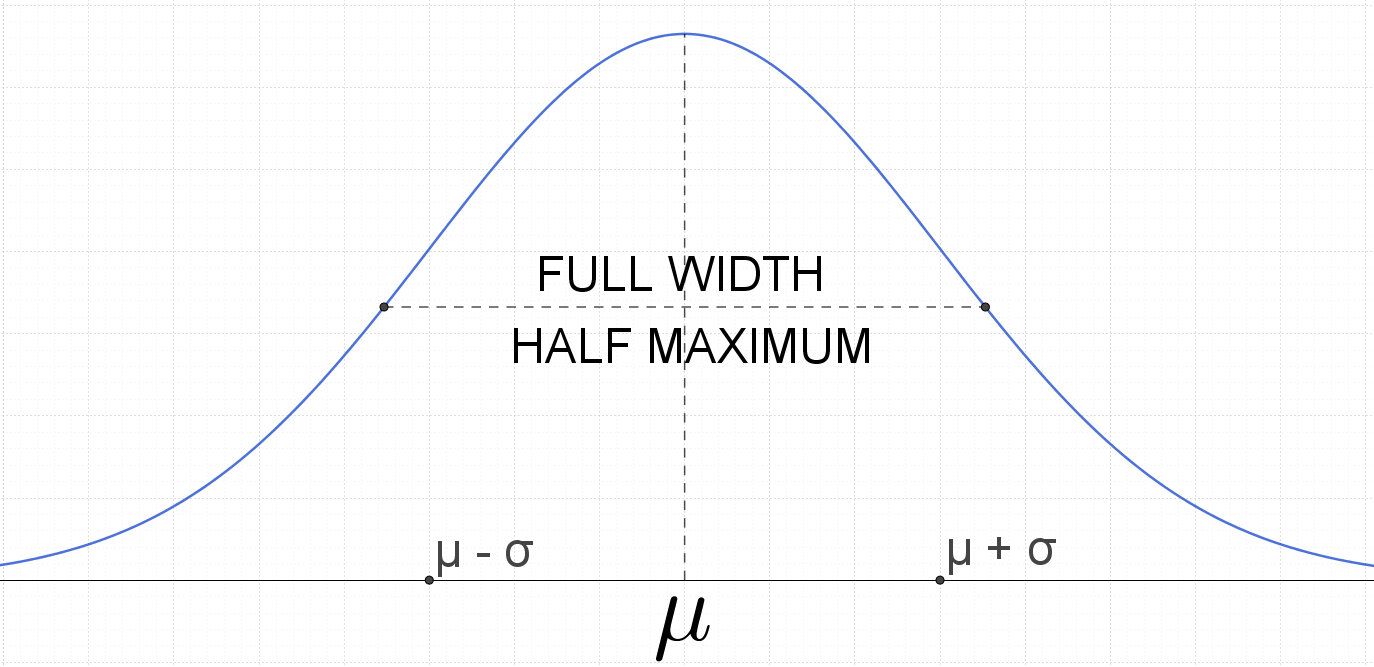
\includegraphics[scale=0.7]{../normal_distribution}
	\end{figure} \\
	Hvor $\mu$ er x-verdien til toppunktet, og $\sigma$ sier noe om bredden til kurven.
	$\mu$ kalles middelverdien, og $\sigma$ kalles standardavviket. For å få en
	visuell forståelse av standardavviket kan man bruke FWHM, "Full width half maximum":
	Forholdet mellom FWHM og standardavviket er
	$$\sigma = \frac{\text{FWHM}}{2\sqrt{2\ln{2}}}$$
	Utldeningen av dette forholdet er i \ref{FWHM}.
	\vspace{0.25cm}
	En annen viktig sannsynlighetsfordeling er Maxvell-Boltzmanns fordelingsfunksjon
	for absolutthastighet:
	$$
		P(v) = \left(\sqrt{\frac{m}{2\pi k T}}\right)^3 e^{-\frac{1}{2}\frac{mv^2}{kT}} 4\pi v^2
	$$
	Denne likner på Maxvell-Boltzmanns fordelingsfunksjon for hastighetskomponenter,
	men på grunn av det siste leddet, $4\pi v^2$, er det ikke en normaldistrobusjon.
	Den er likevel fortsatt en sannsynlighetsfordeling, $\int\limits_{0}^{\infty} P(v)\ dv = 1$.
	Fra Maxvell-Boltzmanns fordelingsfunksjon kan man utlede noen viktige formler: \\
	\\
	Gjennomsnittshastigheten i en gass: \\
	\ $\left<v\right> = \sqrt{\frac{8kT}{\pi m}}$ (\ref{avgSpeed}) \\
	\\
	Den ideelle gassloven: \\
	\ $P = nkT$ (\ref{idealGass}) \\
	\\
	Gjennomsnittsenergien i en gass: \\
	\ $\left<E\right> = \frac{3}{2}kT (sick ref)$

	\vspace{0.5cm}

	Om man skal simulere partikkler i en boks eller en rakettoppskytning trener man
	en numerisk måte å gjøre om akselerasjon til hastighet og hastighet til position.
	Vi vet at gjennomsnittshastighet er endring i position over tid. Fra dette kan
	vi få et uttrykk for endring i position. \\
	$\bar{v} = \frac{\Delta x}{\Delta t} \implies \Delta x = \bar{v}\Delta t \implies x_1 = x_0 + \bar{v}\Delta t$. \\
	Dette antar at hastigheten er konstant. For partiklene i boksen stemmer det,
	men for rakketten må vi få med akselerasjon. Kan utlede et liknende uttrykk for akselerasjonen: \\
	$\bar{a} = \frac{\Delta v}{\Delta t} \implies \Delta v = \bar{a}\Delta t \implies v_1 = v_0 + \bar{a}\Delta t$.
	Vi får altså to likninger som beskriver bevegelsen til raketten:
	\begin{align*}
		v_1 &= v_0 + \bar{a}\Delta t \\
		x_1 &= x_0 + v_1\Delta t
	\end{align*}
	Denne måten å løse bevegelseslikningene kalles Euler-Cromer metoden.
	Eulers metode er liknende, men der oppdateres $x_1 med v_0$, som er litt mindre
	nyaktig. Det er fortsatt antatt konstant akselerasjon, som i rakettoppskytningen
	ikke stemmer, men når tidssteget $\Delta t$ blir like nok vil akselerasjonen
	oppføre seg som om den er konstant.

	\vspace{0.5cm}

	For å forstå hvordan en rakett beveger seg oppover trenger man å vite om newtons lover.
	Newtons andre lov, $\vec{F} = \frac{d\vec{p}}{dt}$ sier oss at kraften, F, er endringen
	i bevegelsesmengde, p, over tid. Når en partikkel skytes ut av rakettmotoren minker
	bevegelsesmengden inne i motoren, som vil si at det virker en kraft nedover på gassmolekylene
	i motoren. Vi vet at denne kraften må komme fra selve raketten, fordi dette er egentlig bare
	kraften fra veggene i motoren på gassmolekylene, og denne kraften er netto nedover
	siden der er like mye vegg loddrett på alle sider, men mer vegg horisontalt i øvre del av
	motoren enn nedre. Fra newtons 3. lov har vi at alle krefter har en lik og motsatt
	rettet motkraft, så når gassmolekylene blir påvirket av en kraft nedover fra selve raketten,
	vil selve raketten bli påvirket av en kraft oppover, og raketten vil lette hvis denne
	kraften er større enn gravitasjonen.

	\vspace{0.5cm}

	Når raketten skal ut i bane rundt planeten må vi bruke tyngdekraften gitt ved
	newtons tyngdekraftslov
	$$
		\vec{F} = \gamma\frac{Mm}{r^2}\hat{r}
	$$
	hvor $\gamma$ er gravitasjonskonstanten, $M$ er massen til planeten, $m$ er massen
	til raketten, $r$ er lengden til vektoren fra planeten til raketten, og $\hat{r}$ er
	retningen til vektoren fra planeten til raketten.

	For å finne ut om raketten klarer å lette og videre komme ut i verdensrommet må vi
	finne ut om den når unnslipningsfarten. Unnslipningsfarten er den farten
	som gir nok kinetisk energi til at raketten kan komme fullstendig ut av planetens gravitasjonsfelt.
	Altså den farten raketten må ha for å komme til dit $r\rightarrow\infty$.
	Raketten må altså ha mer kinetisk energi enn gravitasjonell potensiell energi.

	Så hvis vi har en rakett med masse m og en planet med masse M er unnslipningsfarten:
	$$
		E_k + E_p = 0
	$$
	der $E_p$ kan utledes fra
	$$
		\vec{F}_G = -\nabla E_p
  $$
	slik at den blir
	$$
		E_p = -\gamma \frac{mM}{r}
	$$
  Da har vi at
	\begin{align*}
		E_k &= E_p\\
		\frac{1}{2}mv^2 &= \gamma\frac{mM}{r}\\
    v&=\sqrt{2\gamma\frac{M}{r}}
	\end{align*}
	der r er planetens radius.


\section{Method}
	Først og fremst kan vi se på hvordan vi simulerer bevegelsen til gassmolekylene
	i motoren. Vi tenker oss at rakketdrivstoffet er ren H2-gass, og at motoren har
	en temperatur på $3000$ Kelvin. For å gjøre simuleringen enklere antar vi at H2-gassen
	er en ideell gass, altså at H2-molekylene ikke interagerer med hverandre, dette stemmer
	ikke helt, men det gør at simuleringsalgoritmen er $O(n)$ istedenfor $O(n^2)$. Vi
	må likevel gjøre at rakettmotoren består av veldig mange veldig små bokser, og
	simulere atomene i en sånn boks, for å kunne simulere en rimelig molekyltetthet
	og mange nok tidssteg for å få et godt resultat. Vi teker oss derfor at
	vi har en terningformet boks med sidelengder $L = 10^{-6}$ m med 100000 atomer. \

	Vi startet med å gi hvert molekyl en tilfeldig intialposisjon etter
	lineær distibusjon og en tilfeldig initialhastighet etter gaussisk
	sannsynlighetsfordeling. Maxwell-Boltzmanns sannsynlighetsfordeling (se teoridel) gir oss
	inndelingen av initialhastighetene. For en temperatur på $3000$ K og H2-molekyler
	med en masse på $3.35 \cdot 10^{-27}$ kg har hastighetskomponentene et standardavvik
	på $\sigma = \sqrt{\frac{kT}{m}} = \sqrt{\frac{1.38 \cdot 10^{-27} \cdot 3000}{3.35 \cdot 10^{-24}}} \approx 3517$ \

	\vspace{0.5cm}

	Når man har funnet initialhastigheten og initialposisjonene kan man bruke Eulers
	metode til å simulere bevegelsen til partiklene numerisk:
		$$\vec{r}_{i+1} = \vec{r}_{i} + \vec{v}_i\Delta t$$
	Vi antar at det ikke virker noen gravitasjon på hvert enkelt gassmolekyl i
	boksen, ettersom et hydrogenmolekyl veier så lite at gravitasjonskraften på det er
	neglisjerbar. Dette, sammen med at molekylene ikke kolliderer, betyr at
	molekylene har konstant hastighet helt fram til de kolliderer
	med en av veggene. Vi antar at disse kollisjonene er elastiske,
	altså vil hastigheten i den retningen som kolliderer med veggen ganges med -1.
	Siden vi simulerer for et og et tidssteg kan vi sjekke når partiklene havner uten for veggen
	for hvert tidssteg, og snu hastigheten slik at de går bort fra veggen.
	Da er det slik at hvis veggen som molekylet kolliderer med ligger i for eksempel
	yz-planet så blir hastighetskomponenten i x-retning snudd. Her er valget av
	tidsstegstørrelse viktig, hvis tidsstegene er for store vil molekylene bevege
	seg langt ut av boksen før hastighetskomponenten blir snudd, som kan føre til
	unyaktighet og uventet oppførsel. Gitt et standardavvik på 3517 er det svært
	få moleyler som har hastighetskomponenter større enn 10000 (0.45 \% for å være presis).
	Bruker vi den hastigheten som en øvre grense, kan vi finne tiden det tar for at et
	rastk moleky beveger seg fra en sigen av boksen til den andre:
	$$t = \frac{s}{v} = \frac{10^{-6}\text{ m}}{10^{4}\text{ m/s}} = 10^{-10} \text{ s}$$
	Vi ønsker at et raskt molekyl
	skal bevege seg fra en side av boksen til en annen på N steg, så
	tidsstegstørrelsen vi trenger er $\frac{10^{-10}}{N}$ s. Vi valgte $N = 20$,
	altså $\Delta t = 0.5 \cdot 10^{-11}$, basert
	på en balanse mellom presisjon og simuleringshastighet. Når vi plottet bevegelsen
	til et av molekylene med $N = 20$ så det slik ut:
	\newpage
	\begin{figure}
		\centering
		\caption{Bevegen til et hydrogenmolekyl}
		\makebox[0.5\textwidth][c]{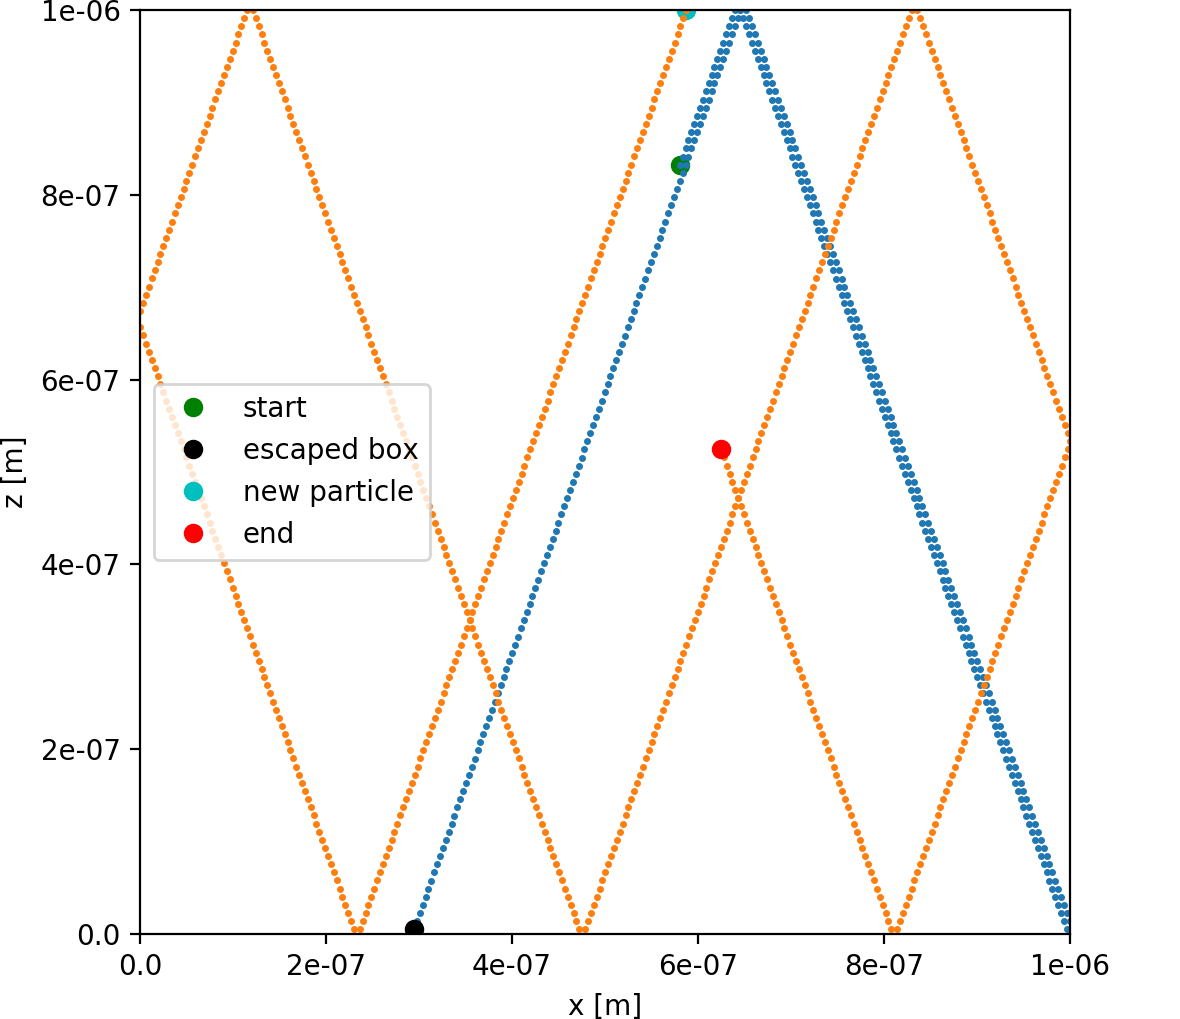
\includegraphics[scale=0.23]{../box_position-stripped}}
	\end{figure}
	Vi så at molekylet ikke kom for langt inn i veggen, og bestemte oss for å ikke
	bruke mer tid på å finpusse tidsstegstørrelsen. Dette plottet viser også at
	molekylet faller ut av boksen og et nytt molekyl kommer inn, som skal forklares
	senere.

	\vspace{0.5cm}

	Videre må vi lage et hull i bunnen av boksen slik at molekylene slipper ut og
	vi får en kraft som dytter raketten oppover. For å sjekke om et molekyl har kommet
	ut av boksen, sjekker vi da om koordinatene ligger både innenfor hullet, og under boksen.
	Man kan prøve seg litt fram med størrelsen på hullet slik at ikke for mye av gassen
	vi har tilgjengelig slipper ut for fort og slik at vi får en stor nok oppdriftskraft.
	Når vi finner ut hvor mange partikler som har gått ut av boksen i et tidssteg
	så kan man finne ut hvilken fart de hadde og dermed endringen i bevegelsesmengde
	ved dette tidssteget. Over en viss tidsperiode får man da endring i bevegelsesmengde over tid,
	som gir oss kraften som virker på raketten ved hjelp
	av Newtons andre lov. Det er også viktig at trykk og temperatur holder seg konstant
	i boksen slik at vi får en kontinuerlig oppdrift, da må vi etterfylle med molekyler
	fra drivstofftanken. Siden de molekylene som slipper ut først mest sannsynlig har
	større hastighet siden de beveger seg mest vil temperaturen i boksen synke hvis
	vi legger til et molekyl med en tilfeldig generert hastighet (fortsatt ved samme
  temperatur som i boksen), derfor ga vi de molekylene som kommer inn fra drivstofftanken
	samme hastighet som det som falt ut, slik at temperaturen holdes konstant. Vi gjorde det slik at de nye
	molekylene da har initialposisjon ved toppen av motoren siden det er der drivstofftanken er.

	Siden det må virke en kraft fra raketten på gassmolekylene for at motoren skal miste
	bevegelsesmengde må det ifølge Newtons 3. lov som nevnt i teoridelen virke en motkraft
	som er like stor og motsatt rettet som virker på raketten. Siden vi regner ut endring
	i bevegelsesmengde per tidssteg for hvert tidssteg kan vi også regne ut denne
	kraften for hvert tidssteg og fra Newtons andre lov akselerasjonen oppover per
	tidssteg. Hvis vi også da tar i betraktning gravitasjonen på raketten og drivstoffet
	og hvor mye massen endres idet mer drivstoff slippes ut kan vi numerisk beregne
	bevegelsen til raketten. Til dette brukte vi Euler-Cromers
	metode til å regne ut hastighet og posisjon:
	\begin{align*}
		\vec{v}_{i+1} &= \vec{v}_i + \vec{a}_i\Delta t \\
		\vec{r}_{i+1} &= \vec{r}_i + \vec{v}_{i+1}\Delta t
	\end{align*}
	Målet er å skyte opp raketten, som vil si å få den til å gå så raskt at den når
	unnslipningshastigheten, som er forklart i teoridelen.
	Vi må først finne unnslipningshastigheten for planeten vår: \\
	Vi har fra \ref{solartable} at planeten har radiue $r = 9.572\cdot10^6$ m og
	masse $M = 1.82\cdot10^{25}$ kg, finner unnslipningshastigheten:
	\begin{align*}
		v &= \sqrt{\frac{2GM}{r}}\\
		&= \sqrt{\frac{2\cdot 6.67\cdot10^{-11}\frac{\text{ m}^3}{\text{ kgs}^2}\cdot1.82\cdot10^{25}\text{ kg}}{9.572\cdot10^6\text{ m}}}\\
		&= 15.93\text{ km/s}
	\end{align*}
	Vi definerer altså å skyte opp raketten som å gi den en hastighet større enn $15.93\text{ km/s}$.
	Når vi skal skyte opp raketten må vi ta hensyn til initialhastigheten til romskipet vårt. Ettersom den er
	på en roterende planet vil den ha en hastighet som avhenger av rotasjonshastigheten
	til planeten, radiusen til planeten og hvor på planeten raketten er. På ekvator
	er initialhastigheten størst, og på polene er initialhastigheten minst. Vi skyter
	derfor raketten opp på et punkt på ekvator, sånn at vi trenger minst mulig ekstra
	hastighet for å nå unnslipningshastigheten. Med verdiene til planeten vår fra
	tabell 1 har vi at rotasjonshastigheten er $\omega = 6.38\cdot10^{-5}\text{ s}^{-1}$.
	Dette gir en initialhastighet (i rotasjonsretningen) $v = \omega \cdot r=6.38\cdot 10^{-5}\text{ s}^{-1} \cdot9.572 \cdot 10^6\text{ m} = 611$ m/s. \\
	Vi definerer startspunktet til romskipet som $(0, 0, r)$ hvor $r$ er radiusen til
	planeten. Vi har altså definert x-aksen til å gå langs ekvator i rotasjonsretningen,
	z-aksen til å gå rett oppover i radiell rettning, og z-aksen til å gå normalt på
	x-aksen og z-aksen. Det vil si at initialhastigheten til rommskipet er i x-retning,
	og kraften fra motoren er i z-retning. I en ekte rakettoppskytning vil raketten
	bøye seg i rotasjonsretningen, men vi antar her at raketten er helt parallell med
	z-aksen hele tiden, og at all akselerasjon foregår i z-retning. Dette er fordi at
	vi ikke har lært hvordan en ekte rakettoppskytning fungerer.

\section{Results}
\section{Discussion}
\section{Conclusion}

\appendix
\section{Utledning}
	\subsection{Utleding av forholdet mellom FWHM og standardavviket}\label{FWHM}
	Skal vise at
	$$\sigma = \frac{\text{FWHM}}{2\sqrt{2\ln{2}}} \implies \text{FWHM} = 2\sqrt{2\ln{2}}\sigma$$
	Toppunktet til en normalkurve er når $x=\mu$. "Half maximum" er derfor $\frac{P(\mu)}{2}$
	(hvor P(x) er normalfunksjonen). "Half maximum" er altså:
	$$
	\frac{P(\mu)}{2} = \frac{1}{2}\frac{1}{\sqrt{2\pi}\sigma}e^{-\frac{1}{2}\left(\frac{\mu - \mu}{\sigma}\right)^2}
	= \frac{1}{2\sqrt{2\pi}\sigma}
	$$
	\\
	Trenger så å finne x-verdien hvor x="Half maximum", løser likningen $P(x) = \frac{P(\mu)}{2}$:
	\begin{align*}
		\frac{1}{\sqrt{2\pi}\sigma}e^{-\frac{1}{2}\left(\frac{x-\mu}{\sigma}\right)^2} &= \frac{1}{2\sqrt{2\pi}\sigma} \\
		e^{-\frac{1}{2}\left(\frac{x-\mu}{\sigma}\right)^2} &= \frac{1}{2} \\
		-\frac{1}{2}\left(\frac{x-\mu}{\sigma}\right)^2 &= \ln{\frac{1}{2}} \\
		\left(\frac{x-\mu}{\sigma}\right)^2 &= 2\ln{2} \\
		\left(x - \mu\right)^2 &= 2\ln{2}\sigma^2 \\
		x - \mu &= \pm\sigma\sqrt{2\ln{2}} \\
		x &= \underline{\mu \pm \sigma\sqrt{2\ln{2}}} \\
	\end{align*}

	"Full width" er max(x) - min(x):
	\begin{align*}
		&\ \ \ \ \ \left(\mu + \sigma\sqrt{2\ln{2}}\right) - \left(\mu - \sigma\sqrt{2\ln{2}}\right) \\
		&= \sigma\sqrt{2\ln{2}} + \sigma\sqrt{2\ln{2}} + \mu - \mu \\
		&= \underline{2\sqrt{2\ln{2}}\sigma}
	\end{align*}
	\\
	"Full width" for "Half maximum" er FWHM, altså er $\text{FWHM} = 2\sqrt{2\ln{2}}\sigma \ \ \square$

	\subsection{Utleding av gjennomsnittshastigheten til en gass}\label{avgSpeed}
	Skal vise at
	$$\left<v\right> = \sqrt{\frac{8kT}{\pi m}}$$
	Har at
	$$\left<v\right> = \int\limits_0^{\infty}vP(v)\ dv \text{, } P(v) = \left(\sqrt{\frac{m}{2\pi k T}}\right)^3 e^{-\frac{1}{2}\frac{m v^2}{k T}}4\pi v^2$$
	Løser integralet:
	\begin{align*}
		\left<v\right> &= \int_0^{\infty}v \left( \left(\sqrt{\frac{m}{2\pi k T}}\right)^3 e^{-\frac{1}{2}\frac{m v^2}{k T}}4\pi v^2 \right) dv \\
		&\ \ \ \ \ \ u = v^2 \implies du = 2vdv \implies dv = \frac{du}{2v} \\
		&= 4\pi \left(\sqrt{\frac{m}{2\pi k T}}\right)^3 \frac{1}{2} \int_0^{\infty} e^{-\frac{1}{2}\frac{m u}{k T}} u\ du \\
		&= 4\pi \left(\sqrt{\frac{m}{2\pi k T}}\right)^3 \frac{1}{2}\int_0^{\infty} ue^{-Cu}\ du\ \text{, }\ C = \frac{1}{2}\frac{m}{k T} \\
		&\ \ \ \ \ \ t = Cu \implies u = \frac{t}{C},\ dt = Cdu,\ du = \frac{dt}{C} \\
		&= 4\pi \left(\sqrt{\frac{m}{2\pi k T}}\right)^3 \frac{1}{2} \frac{1}{C^2}\int_0^{\infty} te^{-t}\ dt \\
		&= 4\pi \left(\sqrt{\frac{m}{2\pi k T}}\right)^3 \frac{1}{2} \frac{1}{\left(\frac{1}{2}\frac{m}{k T}\right)^2} \cdot 1 \\
		&=\sqrt{\frac{8kT}{\pi m}} \ \ \square
	\end{align*}

	\subsection{Utledning av trykket til en ideell gass}\label{idealGass}
	Skal vise at $$P=nkT$$ ut i fra integralet
	$$
	P=\frac{1}{3}\int_{0}^{\infty}pvn(p)dp
	$$
	Hvor $n(p)=nP(p)$ er antalltettheten
	Løser integralet
	\begin{align*}
	  P&=\frac{1}{3}\int_{0}^{\infty}pvn(p)dp\\
		P(v)&=(\frac{m}{2\pi kT})^{\frac{3}{2}}e^{-\frac{mv^2}{2kT}}4\pi v^2\\
		p&=mv\\
		P(p)&=(\frac{m}{2\pi kT})^{\frac{3}{2}}e^{-\frac{p^2}{2kTm}}4\pi\frac{p^2}{m^2}\\
		P&=\frac{1}{3}\int_{0}^{\infty}pvn(p)dp\\
		&=\frac{1}{3}n\int_{0}^{\infty}\frac{p^2}{m}(\frac{m}{2\pi kT})^{\frac{3}{2}}e^{-\frac{p^2}{2kTm}}4\pi\frac{p^2}{m^2}dp\\
		&=\frac{4\pi}{3}n(\frac{m^3}{(2\pi kT)^3m^6})^{\frac{1}{2}}\int_{0}^{\infty}e^{-\frac{p^2}{2kTm}}p^4dp\\
		u&=\frac{p^2}{2kTm}\\
		\frac{du}{dp}&=\frac{p}{kTm}\\
	  dp&=\frac{mkT}{p}du\\
		p&=\sqrt{2mkTu}\\
  \end{align*}
	\newpage %% OBS! fjærn denne kanskje
	\begin{align*}
		&\frac{4\pi}{3}n(\frac{m^3}{(2\pi kT)^3m^6})^{\frac{1}{2}}\int_{0}^{\infty}e^{-\frac{p^2}{2kTm}}p^4dp\\
		&=\frac{4\pi}{3}n(\frac{m^3}{(2\pi kT)^3m^6})^{\frac{1}{2}}mkT(2mkT)^{\frac{3}{2}}\int_{0}^{\infty}e^{-u}(u)^{\frac{3}{2}}dp\\
		&=\frac{4\pi}{3}n(\frac{m^3}{(2\pi kT)^3m^6})^{\frac{1}{2}}mkT(2mkT)^{\frac{3}{2}}\frac{3}{4}\sqrt{\pi}\\
		&=nkT
	\end{align*}
\end{document}
